\subsection{Sliding Rod}
\label{sec:sliding_rod}

This case is particularly interesting as it leads to impact without collision
\cite[\S 5.3]{bib:pfeiffer1996multibody}. A rod initially angled with the ground
makes single-point contact with a horizontal velocity (see Fig.
\ref{fig:sliding_rod_setup}). As it slides, friction rotates the rod into the
ground, increasing the normal force. Under specific conditions, both normal and
frictional forces intensify, potentially leading to a singularity in
acceleration-level formulations with Coulomb friction known as Painlev\'e's
paradox, where forces become infinite. This problem is resolved in the discrete
setting, where finite impulses and discrete velocity changes are allowed.
Physically, bodies aren't perfectly rigid --- they deform, vibrate, and may
even undergo plastic (permanent) deformations. Nonetheless, a rapidly increasing
contact force develops an impact that makes the rod jam into the ground and jump
into the air. The rod measures $0.5\text{ m}$ in length, $1\text{ cm}$ in
diameter, and has a mass of $0.3\text{ kg}$.

\begin{figure}[!h]
    \centering
    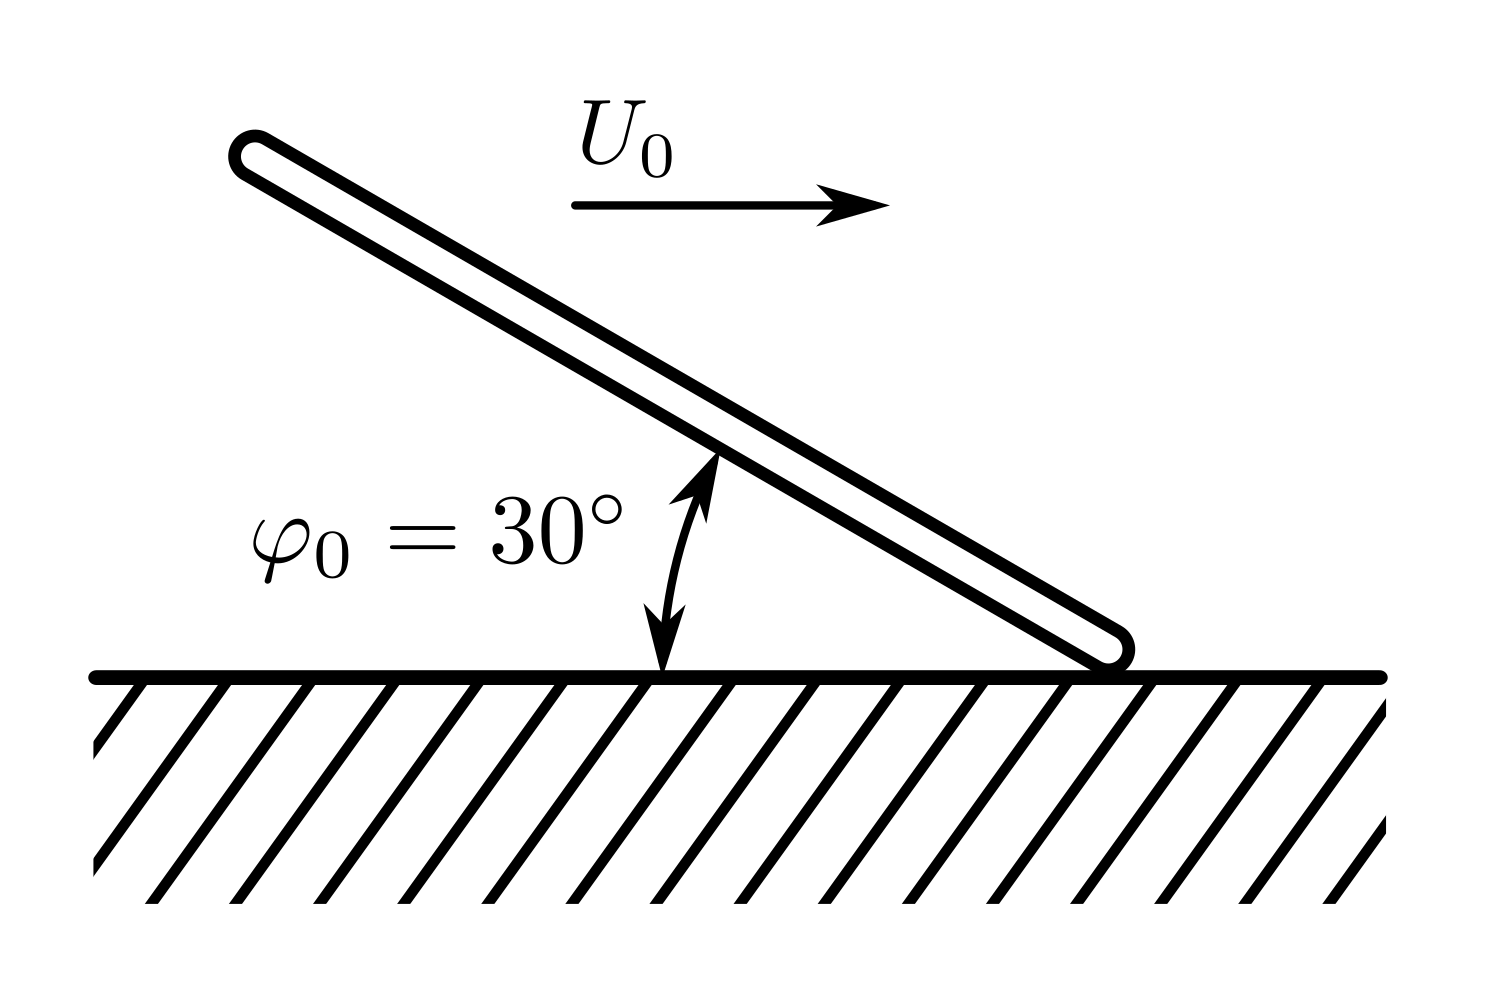
\includegraphics[width=0.55\columnwidth]{figures/TestCases/SlidingRod/sliding_rod_schematic.png}
    \caption{Sliding rod. Initially forming an angle $\varphi_0$ with the ground
    and with horizontal velocity $U_0$. Friction makes the rod rotate clockwise.
    The contact force increases until the rod jams into the ground, causing the
    rod to jump into the air.}
    \label{fig:sliding_rod_setup}
\end{figure}

Analytical analysis \cite[\S 5.3]{bib:pfeiffer1996multibody} shows that the
singularity occurs when $\mu>4/3$ and the initial kinetic energy overcomes
potential energy as the rod's center of gravity rises and friction dissipates
energy. We set $\mu=2.3$, a $30^\circ$ initial angle (Fig.
\ref{fig:sliding_rod_setup}), and an initial horizontal speed $U_0=10\text{
m}/\text{s}$.

Using a reference solution with a time step of $\delta t=10^{-7}\text{ s}$ and no
normal force dissipation, we observe that the rod rotates upward and jams into
the ground upon contact as expected. All three models yield similar results, as
the compliant model is identical in the absence of dissipation, differing only
in friction regularization. Pre-impact forces oscillate based on ground
compliance, and impact location is nearly identical across models (
Fig. \ref{fig:rod_contact_force_no_diss}) despite being very sensitive to model
parameters.

\begin{figure}[!h]
    \centering
    %trim={<left> <lower> <right> <upper>}
    \adjincludegraphics[height=0.375\columnwidth,trim={0 0 {0.05\width} 0},clip]{figures/TestCases/SlidingRod/SteelRod/contact_forces_no_diss.png}
    \adjincludegraphics[height=0.375\columnwidth,trim={0 0 {0.05\width} 0},clip]{figures/TestCases/SlidingRod/SteelRod/contact_forces_no_diss_zoom.png}
    \caption{\label{fig:rod_contact_force_no_diss} Contact forces in the case with zero
    dissipation. The figure on the right shows a close-up near the impact.}
\end{figure}

Figure \ref{fig:rod_contact_velocity_no_diss} shows the contact point moves
into the ground due to large contact forces until the tangential component of
the velocity goes to zero and the rod jams into the ground. During stiction
$\Vert\vf{v}_t\Vert<v_s$ for a finite period of about $0.2\text{ ms}$.

\begin{figure}[!h]
    \centering
    %trim={<left> <lower> <right> <upper>}
    \adjincludegraphics[height=0.375\columnwidth,trim={0 0 {0.05\width} 0},clip]{figures/TestCases/SlidingRod/SteelRod/contact_velocities_no_diss.png}
    \adjincludegraphics[height=0.375\columnwidth,trim={0 0 {0.05\width} 0},clip]{figures/TestCases/SlidingRod/SteelRod/contact_velocities_no_diss_zoom.png}
    \caption{\label{fig:rod_contact_velocity_no_diss} Contact velocities in the case with zero
    dissipation. The figure on the right shows a close-up near the impact.}
\end{figure}

We run the simulation with Hunt \& Crossley dissipation $d=0.2\text{ s}/\text{m}$
and relaxation time $\tau_d = 4.0\times{10}^{-6}\text{ s}$. These low
dissipation values have minimal effect on the time of impact for the Lagged model,
our reference solution, as seen in Figs. \ref{fig:rod_contact_force} and
\ref{fig:rod_contact_velocity}. However, Similar and SAP models predict shifted
impact times—earlier for Similar, later for SAP. Although their contact forces and
velocities differ significantly, we choose $\tau_d$ for SAP to match the shift in time
of impact observed in the Similar model, albeit in the opposite direction.
Compliance modulation in Similar becomes evident in Fig.
\ref{fig:rod_contact_force}, where we observe a frequency shift on the force
oscillations. This is caused by the larger effective stiffness of the model
during sliding, $k_\text{eff}=k\,(1+\mu\Vert\vf{v}_t\Vert\,d)$.

\begin{figure}[!h]
    \centering
    %trim={<left> <lower> <right> <upper>}
    \adjincludegraphics[height=0.375\columnwidth,trim={0 0 {0.05\width} 0},clip]{figures/TestCases/SlidingRod/SteelRod/contact_forces.png}
    \adjincludegraphics[height=0.375\columnwidth,trim={0 0 {0.05\width} 0},clip]{figures/TestCases/SlidingRod/SteelRod/contact_forces_zoom.png}
    \caption{\label{fig:rod_contact_force} Contact forces in the case
    with dissipation. The figure on the right shows a close-up near the impact.}
\end{figure}

A convergence analysis with and without dissipation is shown in Fig.
\ref{fig:rod_convergence}, using time steps $\delta t=\{6.4\times 10^{-4},
1.6\times 10^{-4}, 4.0\times 10^{-5}, 1.0\times 10^{-5}\}\text{ s}$. Without
dissipation, SAP and Similar model solutions are indistinguishable. The Lagged
model exhibits the largest error at the largest time step. revealing a limitation:
its lagged normal force affects Coulomb friction modeling in rapidly changing
scenarios, even missing impacts when $\delta t > 10^{-3}\text{ s}$. However, it
achieves first-order convergence with smaller steps. Similar trends occur with
non-zero dissipation, though the curves diverge as time of impact predictions shift.

\begin{figure}[!h]
    \centering
    %trim={<left> <lower> <right> <upper>}
    \adjincludegraphics[height=0.375\columnwidth,trim={0 0 {0.05\width} 0},clip]{figures/TestCases/SlidingRod/SteelRod/contact_velocities.png}
    \adjincludegraphics[height=0.375\columnwidth,trim={0 0 {0.05\width} 0},clip]{figures/TestCases/SlidingRod/SteelRod/contact_velocities_zoom.png}
    \caption{\label{fig:rod_contact_velocity} Contact velocities in the case
    with dissipation. The figure on the right shows a close-up near the impact.}
\end{figure}


\begin{figure}[!h]
    \centering
    %trim={<left> <lower> <right> <upper>}
    \adjincludegraphics[height=0.375\columnwidth,trim={0 0 {0.05\width} 0},clip]{figures/TestCases/SlidingRod/SteelRod/position_errors_no_diss.png}
    \adjincludegraphics[height=0.375\columnwidth,trim={0 0 {0.05\width} 0},clip]{figures/TestCases/SlidingRod/SteelRod/position_errors.png}
    \caption{\label{fig:rod_convergence} Convergence in positions with
    time step. Case without dissipation (left) and with dissipation (right).}
\end{figure}
